\newpage
\subsection{Einteilung der Funktionen}

Funktionen werden in verschiedenen Arten unterschieden:\\
\begin{enumerate}
    \item Funktion 1.Grades (Lineare Funktion):\textcolor{red}{$f(x)=a+x^1+d$}
    \item Funktion 2.Grades (Quadratische Funktion):\textcolor{blue}{$f(x)=ax^2+bx^1+d$}
    \item Funktion 3.Grades (Kubische Funktion):\textcolor{violet}{$f(x)=ax^3+bx^2+cx^1+d$}
\end{enumerate}


\hfill \break
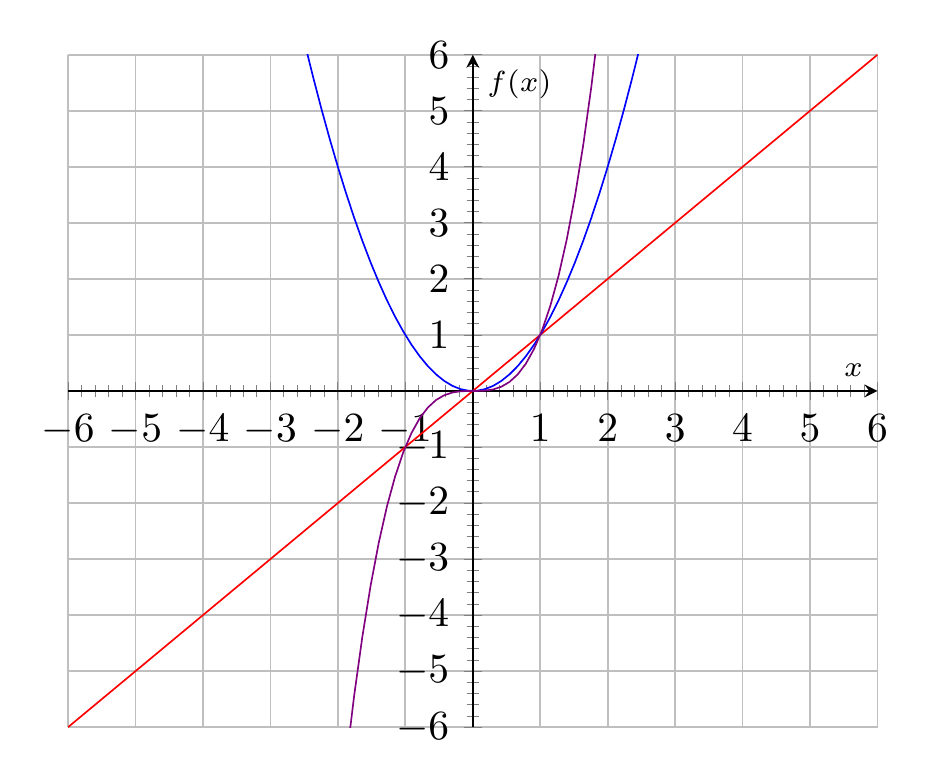
\begin{tikzpicture}[scale=1.5]
    \begin{axis}%
        [
            grid=major,
            xtick={-7,-6,...,7},
            minor x tick num=4, % 4 minor ticks => 5 subintervals
            xmin=-6,
            xmax=6,
            xlabel={\scriptsize $x$},
            axis x line=middle,
            ytick={-6,-5,...,7},
            minor y tick num=4,  % 4 minor ticks => 5 subintervals
            ymin=-6,
            ymax=6,
            ylabel={\scriptsize $f(x)$},
            axis y line=middle,
            no markers,
            samples=100,
            domain=-6:6,
        ]
        \addplot[red] (x,{x});
        \addplot[blue] (x,{x*x});
        \addplot[violet] (x,{x*x*x});
    \end{axis}
\end{tikzpicture}